\documentclass[11pt,a4paper]{article}
\usepackage[margin=2.2cm]{geometry}
\usepackage{float,booktabs,multirow,graphicx,amsmath,amssymb,xcolor,caption,subcaption,enumitem,hyperref}
\usepackage[T1]{fontenc}
\hypersetup{colorlinks=true,linkcolor=blue!50!black,urlcolor=blue!50!black}
\captionsetup{font=small,labelfont=bf}
\setlist{nosep,leftmargin=1.4em}
\newcommand{\best}[1]{\textbf{#1}}
\newcommand{\Lpch}{$\mathcal{L}_{\mathrm{PCH}}$}
\newcommand{\Lrank}{$\mathcal{L}_{\mathrm{rank}}$}
\newcommand{\Lmul}{$\mathcal{L}_{\mathrm{mul}}$}

\title{DMMST: Experimental Results\\[2pt]\large Dynamic Multi-modal Multi-event Survival Transformer}
\date{Results of notebooks 01--11 \quad(\today)}
\author{}

\begin{document}
\maketitle
\tableofcontents
\bigskip

\paragraph{Note on SUPPORT (found after these runs).} The numeric preprocessing used METABRIC's column
layout for every dataset. On SUPPORT, five physiological measurements entered the models unscaled and mean
blood pressure was reduced to a constant. This affects every SUPPORT number on the numeric path in
Tables~\ref{tab:single} and~\ref{tab:disc} (all models alike, including Cox). The parser is fixed
and the SUPPORT experiments are being re-run (notebook 12); METABRIC and all other datasets are unaffected.

\section*{Summary of what we know}
\begin{itemize}
  \item \textbf{The base model is strong.} The transformer with the piecewise-constant-hazard likelihood
        (\Lpch{}) is the best or tied-best model among those we ran on METABRIC, SUPPORT, hsa\_synthetic, EBMT and
        the simulator, with the best calibration among neural models. On METABRIC it matches the published
        PC-Hazard and Cox values; it remains below the published SurvTRACE (0.675 vs.\ 0.691 on METABRIC,
        0.608 vs.\ 0.640 on SUPPORT).
  \item \textbf{It orders events within a patient best among learned models}, measured against the
        simulator's true event times. DeepHit (a competing-risk model) ranks patients well but orders events within
        a patient badly, which supports the paper's general multi-event formulation.
  \item \textbf{The penalty terms do not help.} \Lrank{} and \Lmul{} never improve discrimination, calibration or
        true event ordering; tuned, they become neutral; with the original sharpness ($\sigma=0.1$) they hurt.
  \item \textbf{The within-subject C-index can be gamed.} \Lmul{} raises it above the oracle while making the true
        ordering worse. Proper scores against the true event order are needed to evaluate multi-event models.
  \item \textbf{When a neural model pays off}: Cox is optimal for linear signal and collapses for non-linear
        signal; with few patients ($\le$\,2\,500) Cox and the transformer are comparable, from $\approx$\,5\,000 patients
        the transformer leads clearly.
  \item \textbf{Open}: coded sequences (\S4.2) do not yet beat a bag-of-codes table, the end-to-end LLM (\S3)
        works but is clearly weaker, and continuous vs.\ discretised input is dataset-dependent.
\end{itemize}

%=====================================================================
\section{Setup}
%=====================================================================

\subsection{Datasets}
\begin{center}\small
\resizebox{\textwidth}{!}{\begin{tabular}{lrrll}
\toprule
Dataset & $n$ & events & regime & features \\
\midrule
METABRIC & 1\,904 & 1 & single event & 9 (5 numeric, 4 categorical) \\
SUPPORT & 8\,873 & 1 & single event & 14 (8 numeric, 6 categorical) \\
hsa\_synthetic & 5\,000 & 2 & non-competing & 15 numeric \\
EBMT & 2\,279 & 5 & semi-competing (death censors others) & 4 categorical \\
sim\_* (simulator) & 500--10\,000 & 2--8 & any & 15 numeric, true CIFs known \\
ehrsim / ehrsim2 & 5\,000 & 4 & semi-competing & coded visit histories (age, sex + $\approx$70--80 codes) \\
\bottomrule
\end{tabular}}
\end{center}
The simulator (\texttt{sat/data/simulate.py}) draws Weibull proportional-hazard event times with controllable
event-order spread, shared risk, frailty, non-linearity, censoring and regime; its true cumulative incidence
functions (CIFs) give an \emph{oracle} row. The EHR simulator (\texttt{sat/data/simulate\_ehr.py}) generates
diagnosis, medication, lab and noise codes over 5 years of visits; v2 removes shortcuts so that part of the
risk is only visible in the order, trend and recency of the history.

\subsection{Models}
\begin{itemize}
  \item \textbf{Ours}: numeric-value-embedding transformer + piecewise-constant-hazard head. Loss variants:
        \Lpch{}; $+$\Lrank{} (across patients, Eq.~4); $+$\Lmul{} (within patient, Eq.~5); the paper recipe
        \Lpch{}$+$\Lrank{}$+$\Lmul{}; and $+$MMV (UniSurv mean/variance loss, weight $\lambda_v$).
  \item \textbf{Baselines}: cause-specific Cox PH; DeepHit, DSM and MENSA as published (same transformer
        backbone, their own heads/losses); the oracle (true CIFs) on simulated data.
  \item \textbf{End-to-end LLM} (\S3): DistilGPT2 (pretrained) or a small GPT-2 (from scratch) answering with one
        token per time unit (\texttt{N}, \texttt{C}, \texttt{E}$k$); curves derived from token probabilities.
\end{itemize}

\subsection{Metrics}
\begin{center}\small
\begin{tabular}{p{3.4cm}p{11.6cm}}
\toprule
C$_{td}$ $\uparrow$ & Time-dependent concordance across patients, per event, at the 25/50/75\,\% quantiles
                     (SurvTRACE protocol; multi-event: each event at its own quantiles), averaged. \\
Brier $\downarrow$ & Calibration at the same horizons. \\
Within-subject C $\uparrow$ & Eq.~5 pairs: at the time an event happened, was it ranked more likely than the
                     patient's later or censored events? \emph{Can be gamed} (Section~\ref{sec:true}). \\
True-order C / Brier / log-loss & Simulated data only: predicted $P(T_a<T_b\mid x)$ from each model's curves scored
                     against the true (latent) event times; Brier and log-loss are proper scores (the oracle
                     cannot be beaten in expectation). \\
MAE (uncensored / margin) & Error of the predicted event time in the dataset's unit (METABRIC: months; SUPPORT,
                     EBMT: days; simulator: arbitrary); margin also scores censored patients via a Kaplan--Meier best
                     guess (unreliable on EBMT). \\
\bottomrule
\end{tabular}
\end{center}

\subsection{Protocol}
Each configuration is run with 3--5 seeds; seed $s$ uses initialisation $s$ \emph{and} train/validation/test split
$s$ (60/10/30\,\%). Checkpoints are selected on validation C$_{td}$. Tables report mean $\pm$ sd over seeds;
``paired'' comparisons use the same seed (same split) for both models and give the number of wins and a paired
$t$-test $p$-value. With 5 seeds the smallest attainable Wilcoxon $p$ is 0.0625, so we quote the $t$-test.

\paragraph{Earlier results are superseded.} Before these runs, five bugs were fixed: train/validation were swapped
(models trained on $\approx$10\,\% of the data), Cox ignored categorical features, the ``$+$\Lmul{}'' run never
contained \Lmul{}, checkpoints were selected with a broken C-index, and the split never changed across seeds.

%=====================================================================
\section{Single-event benchmarks: METABRIC and SUPPORT (notebook 03)}
%=====================================================================

\begin{table}[H]\centering\small
\caption{C$_{td}$ (mean over the 25/50/75\,\% horizons) and Brier, 5 splits. ``published'' = SurvTRACE
(Wang \& Sun, 2022) Table~2, averaged over the same three horizons (their 10 runs, different splits).
MAE-unc.\ in months (METABRIC) and days (SUPPORT). SUPPORT columns are affected by the preprocessing issue noted on
page~1 and will be replaced.}
\label{tab:single}
\resizebox{\textwidth}{!}{\begin{tabular}{lcccc@{\hspace{1.2em}}cccc}
\toprule
 & \multicolumn{4}{c}{METABRIC} & \multicolumn{4}{c}{SUPPORT}\\
\cmidrule(lr){2-5}\cmidrule(lr){6-9}
Model & C$_{td}$ & Brier & MAE-unc. & published & C$_{td}$ & Brier & MAE-unc. & published \\
\midrule
Cox PH & 0.625\,$\pm$\,0.027 & 0.180 & 62.2 & 0.629 & 0.555\,$\pm$\,0.004 & 0.203 & 608 & 0.566 \\
DeepHit & 0.670\,$\pm$\,0.013 & 0.189 & 75.4 & 0.657 & 0.599\,$\pm$\,0.005 & 0.218 & 545 & 0.609 \\
DSM & 0.649\,$\pm$\,0.048 & 0.206 & 70.1 & 0.669 & 0.542\,$\pm$\,0.042 & 0.253 & 578 & 0.615 \\
MENSA & 0.650\,$\pm$\,0.027 & 0.188 & 69.2 & -- & 0.581\,$\pm$\,0.026 & 0.212 & 535 & -- \\
SurvTRACE (published only) & -- & -- & -- & 0.691 & -- & -- & -- & 0.640 \\
\midrule
Ours \Lpch{} & \best{0.675}\,$\pm$\,0.014 & \best{0.177} & 69.6 & 0.679$^\dagger$ & \best{0.608}\,$\pm$\,0.005 & \best{0.199} & 573 & 0.626$^\dagger$ \\
Ours $+$\Lrank{} & 0.664\,$\pm$\,0.008 & 0.185 & 66.8 & & 0.608\,$\pm$\,0.009 & 0.204 & 585 & \\
Ours $+$MMV ($\lambda_v{=}0.01$) & 0.666\,$\pm$\,0.011 & 0.190 & 59.0 & & 0.593\,$\pm$\,0.026 & 0.202 & 557 & \\
Ours full, $\lambda_v{=}0.01$ & 0.658\,$\pm$\,0.015 & 0.196 & 57.4 & & 0.608\,$\pm$\,0.007 & 0.204 & 577 & \\
Ours full, $\lambda_v{=}0.1$ & 0.667\,$\pm$\,0.012 & 0.189 & 56.6 & & 0.607\,$\pm$\,0.012 & 0.204 & 556 & \\
Ours full, $\lambda_v{=}1$ & 0.669\,$\pm$\,0.012 & 0.244 & \best{54.1} & & 0.608\,$\pm$\,0.004 & 0.205 & \best{494} & \\
\bottomrule
\multicolumn{9}{l}{\footnotesize $^\dagger$published PC-Hazard (the same head without our transformer); ``full'' = \Lpch{}$+$\Lrank{}$+$\Lmul{}$+$MMV.}
\end{tabular}}
\end{table}

\paragraph{Reading Table~\ref{tab:single}.}
Among the models we ran, our \Lpch{} model is the best on both datasets in discrimination and calibration. On
METABRIC it matches the published PC-Hazard value (0.675 vs.\ 0.679) and Cox matches its published value (0.625
vs.\ 0.629), which validates the evaluation pipeline. On SUPPORT every model sits 0.01--0.02 below its published
value, consistent with different splits. The published SurvTRACE remains ahead (0.691 and 0.640; 0.686 and 0.636
without its multi-task head): our backbone was tuned per dataset on validation over SurvTRACE's own grid (METABRIC: 2 layers,
SUPPORT: 3 layers; hidden size 16, lr \(10^{-3}\)), but our model has no multi-task head and is evaluated
on different splits, so parity with SurvTRACE is not shown. DSM is unstable (sd up to 0.048). Adding \Lrank{} never helps (METABRIC $-0.010$, 0/5
wins; SUPPORT $\pm0$) and worsens Brier in 5/5 splits on both datasets. MMV does what it targets: the error on
observed patients falls from 69.6 to 54.1 months (METABRIC) and 573 to 494 days (SUPPORT) at $\lambda_v=1$, but on
METABRIC Brier rises from 0.177 to 0.244. On SUPPORT, $\lambda_v=1$ is the best trade-off (same C$_{td}$, $-14\,\%$
MAE, $+0.006$ Brier).

%=====================================================================
\section{Multi-event benchmarks (notebook 01, reruns in 07)}
%=====================================================================

\begin{table}[H]\centering\small
\caption{Multi-event datasets, 5 splits (EBMT: 3--5, see text). Within-C = within-subject C-index (gameable);
KM = the same score from population Kaplan--Meier curves (no patient information).}
\label{tab:multi}
\begin{tabular}{lcccccc}
\toprule
 & \multicolumn{3}{c}{sim\_base (4 events)} & hsa (2 events) & \multicolumn{2}{c}{EBMT (5 events)} \\
\cmidrule(lr){2-4}\cmidrule(lr){5-5}\cmidrule(lr){6-7}
Model & C$_{td}$ & Brier & Within-C & C$_{td}$ & C$_{td}$ & Within-C \\
\midrule
Oracle & 0.736 & 0.156 & 0.696 & -- & -- & -- \\
Population KM & -- & -- & 0.580 & -- & -- & 0.837 \\
\midrule
Cox PH & 0.679 & 0.175 & 0.647 & 0.492 & 0.533 & 0.843 \\
DeepHit & 0.712 & 0.230 & \best{0.678} & 0.865 & 0.528 & 0.841 \\
DSM & 0.712 & 0.167 & 0.668 & 0.865 & 0.501 & 0.189 \\
MENSA & 0.701 & 0.172 & 0.649 & 0.865 & 0.504 & 0.465 \\
\midrule
Ours \Lpch{} & \best{0.713} & \best{0.166} & 0.674 & \best{0.867} & \best{0.545} & 0.840 \\
Ours $+$\Lmul{} & 0.700 & 0.172 & 0.666 & 0.846 & 0.535 & 0.880 \\
Ours $+$\Lrank{} & \best{0.713} & 0.180 & 0.639 & 0.868 & 0.543 & 0.838 \\
Ours paper recipe & \best{0.713} & 0.182 & 0.658 & 0.864 & 0.537 & 0.879 \\
Ours full ($+$MMV, $\lambda_v{=}1$) & 0.712 & 0.213 & 0.673 & 0.858 & 0.550 & \best{0.894} \\
\bottomrule
\end{tabular}
\end{table}

\paragraph{Reading Table~\ref{tab:multi}.}
On the simulator our \Lpch{} model is the closest learned model to the oracle (C$_{td}$ 0.713 vs.\ 0.736) with
the best Brier; DeepHit and DSM tie on C$_{td}$ but are worse calibrated. On hsa\_synthetic the signal is purely
non-linear: Cox is at chance (0.49) while all neural models reach $\approx$0.865. On EBMT the four categorical
covariates carry little signal (C$_{td}\approx0.53$--$0.55$ for every model) and the population order of events
is already very predictable (KM within-C 0.837). Adding \Lmul{} lowers C$_{td}$ on sim\_base ($-0.013$, 0/5 wins,
$p=0.002$) and hsa ($-0.021$, 0/5, $p<0.001$). On EBMT it raises within-C from 0.84 to 0.88 (5/5 wins) --- but
EBMT is semi-competing, exactly the setting where Section~\ref{sec:true} shows this metric is gamed. The three
EBMT runs that crashed (fixed, notebook 07) agree with the table (\Lpch{}$+$\Lmul{}: C$_{td}$ 0.537, within-C 0.887;
full: 0.525, 0.901).

%=====================================================================
\section{Is within-subject ordering really improved? (notebook 08)}\label{sec:true}
%=====================================================================

\begin{table}[H]\centering\small
\caption{Within-subject ordering scored against the simulator's \emph{true} event times, 5 splits.
True-order Brier and log-loss are proper scores: no model can beat the oracle in expectation.}
\label{tab:true}
\resizebox{\textwidth}{!}{\begin{tabular}{lccccc@{\hspace{1.2em}}cccc}
\toprule
 & \multicolumn{5}{c}{sim\_base (non-competing)} & \multicolumn{4}{c}{semi-competing} \\
\cmidrule(lr){2-6}\cmidrule(lr){7-10}
Model & C$_{td}$ & Within-C & TO-C & TO-Brier & TO-logloss & C$_{td}$ & Within-C & TO-C & TO-Brier \\
\midrule
Oracle & 0.736 & 0.696 & 0.685 & 0.203 & 0.592 & 0.734 & 0.739 & 0.673 & 0.210 \\
\midrule
Cox PH & 0.679 & 0.647 & 0.624 & 0.227 & 0.645 & 0.679 & 0.716 & 0.623 & 0.227 \\
DeepHit & 0.711 & 0.674 & 0.552 & 0.244 & 0.681 & 0.712 & 0.546 & 0.559 & 0.281 \\
MENSA & 0.709 & 0.664 & 0.653 & 0.218 & 0.626 & 0.708 & 0.715 & 0.644 & 0.221 \\
\midrule
Ours \Lpch{} & \best{0.714} & 0.673 & \best{0.659} & \best{0.215} & \best{0.618} & \best{0.714} & 0.738 & \best{0.658} & \best{0.214} \\
Ours $+$\Lmul{} & 0.709 & 0.671 & 0.657 & 0.220 & 0.630 & 0.703 & \textcolor{red!70!black}{0.787} & 0.633 & 0.228 \\
Ours paper recipe & 0.715 & 0.659 & 0.653 & 0.230 & 0.653 & 0.713 & \textcolor{red!70!black}{0.781} & 0.618 & 0.232 \\
\bottomrule
\multicolumn{10}{l}{\footnotesize TO = true order. Red: above the oracle on the gameable metric while worse on every true-order score.}
\end{tabular}}
\end{table}

\paragraph{Reading Table~\ref{tab:true}.}
This is the decisive test for \Lmul{}. On true-order scores our \Lpch{} model is the best learned model in both
regimes, ahead of MENSA, Cox and DeepHit. Adding \Lmul{} or using the paper recipe makes every true-order score
worse (TO-Brier: 0/5 wins in all four comparisons, $p<0.001$). In the semi-competing regime \Lmul{} raises the
gameable within-C to 0.787 --- \emph{above the oracle's} 0.739 --- while its true-order C falls by 0.025. The loss is
trained on the same pairs the metric counts and learns to reshape the event curves around the terminal event,
which wins those pairs without predicting better. DeepHit has a good C$_{td}$ but the worst true ordering (0.552):
its likelihood assumes one event per patient (competing risks) and is misspecified when events co-occur.

\subsection*{Tuning the penalties}
\begin{table}[H]\centering\small
\caption{Penalty weight and sharpness $\sigma$ tuned on validation C$_{td}$ (split 0), then tested on 5 splits.}
\label{tab:tune}
\begin{tabular}{llcccc}
\toprule
Penalty (data) & chosen setting & & C$_{td}$ & Brier & TO-Brier \\
\midrule
\Lrank{} (METABRIC) & $\sigma{=}0.5$, weight 0.01 & \Lpch{} & 0.6705 & 0.1810 & -- \\
 & & tuned \Lrank{} & 0.6718 & 0.1776 & -- \\
\Lmul{} (sim\_base) & $\sigma{=}0.5$, weight 0.2 & \Lpch{} & 0.7152 & 0.1662 & 0.2148 \\
 & & tuned \Lmul{} & 0.7139 & 0.1661 & 0.2145 \\
\bottomrule
\end{tabular}
\end{table}

\paragraph{Reading Table~\ref{tab:tune}.}
The validation grids ($\sigma\in\{0.1,0.5,1\}$, weight $\in\{0.01,0.05,0.2\}$) both ranked $\sigma=0.1$ --- the
value used everywhere before --- last. With the best setting each penalty becomes indistinguishable from \Lpch{}
(METABRIC 3/5 wins, $p=0.81$). Tuning removes the harm but adds no benefit. Our reading: \Lpch{} is the full
likelihood of the event times, so it already learns the ranking and the order the model can represent; a ranking
penalty can only pull the curves away from that optimum.

%=====================================================================
\section{Simulator sweeps (notebooks 02 and 11)}
%=====================================================================
Each figure varies one simulator setting around the base scenario (3 splits; error bars = sd). The dashed grey
line is the oracle. Panels: within-subject C, C$_{td}$, within-C gain over population KM (and, for notebook 11,
true-order Brier). Notebook 02 ran before the true-order score existed.

\begin{figure}[H]\centering
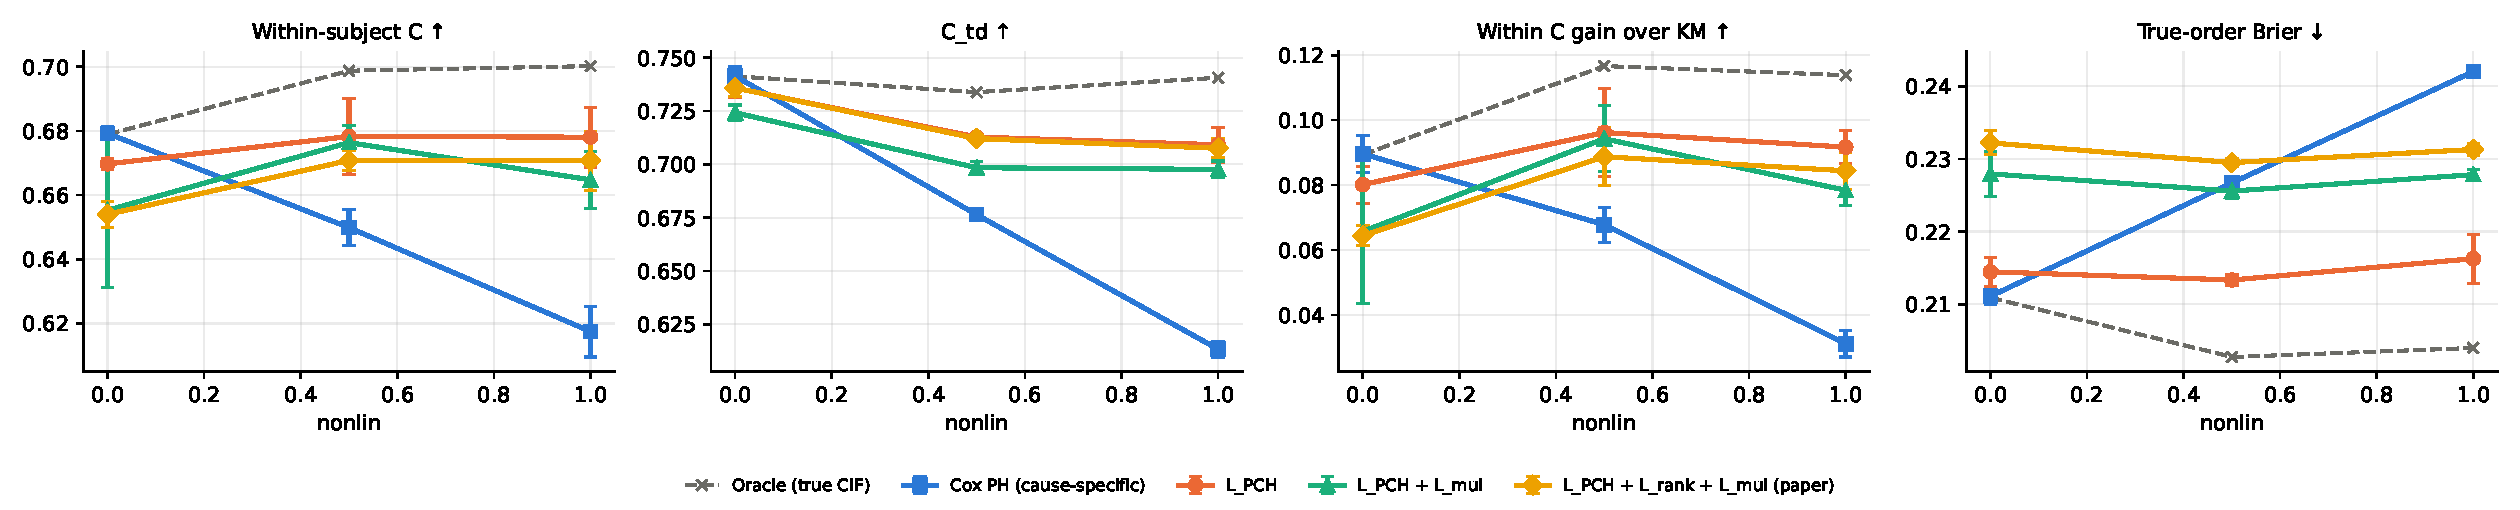
\includegraphics[width=\textwidth]{figures/sweep_nonlin.pdf}
\caption{Non-linearity of the risk (0 = linear, 1 = fully non-linear).}\label{fig:nonlin}
\end{figure}
\paragraph{Figure~\ref{fig:nonlin}.} With a linear signal Cox equals the oracle (C$_{td}$ 0.741) and our model
loses little (0.736). As the signal becomes non-linear Cox collapses (0.613) while ours stays at 0.709 (oracle
0.741). This is the clearest argument for a neural model.

\begin{figure}[H]\centering
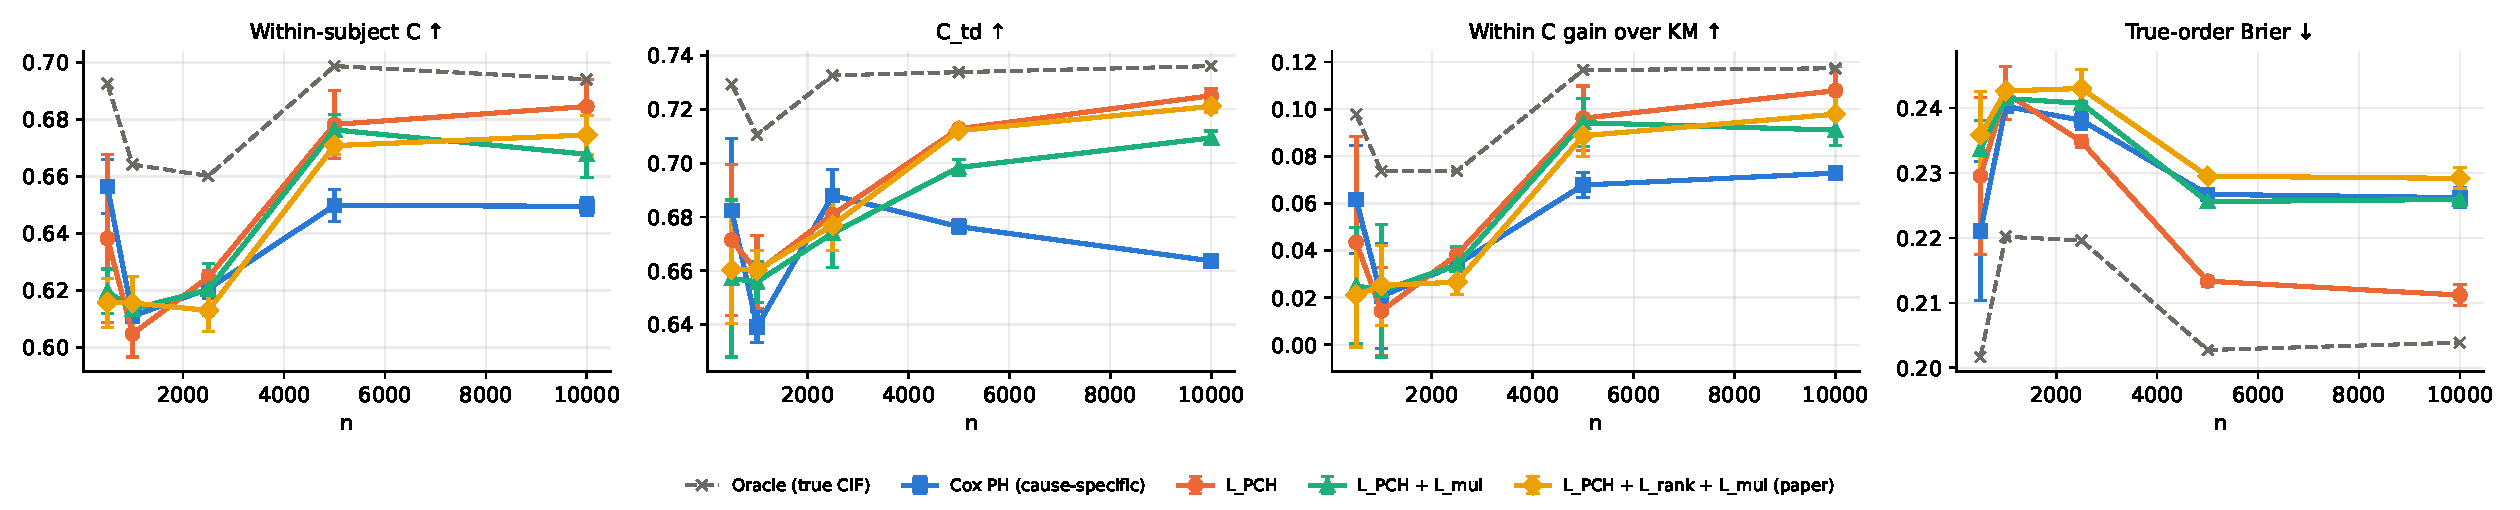
\includegraphics[width=\textwidth]{figures/sweep_n.pdf}
\caption{Training-set size (500 to 10\,000 subjects).}\label{fig:n}
\end{figure}
\paragraph{Figure~\ref{fig:n}.} The gap of our model to the oracle shrinks from 0.058 ($n{=}500$) to 0.011
($n{=}10\,000$); Cox's gap stays 0.05--0.07. Below 5\,000 subjects the two are comparable (Cox ahead at
$n=500$ and $2\,500$, the transformer at $n=1\,000$); from $\approx5\,000$ subjects the transformer leads clearly. Each $n$ is a different random dataset, so the small-$n$ points are noisy.

\begin{figure}[H]\centering
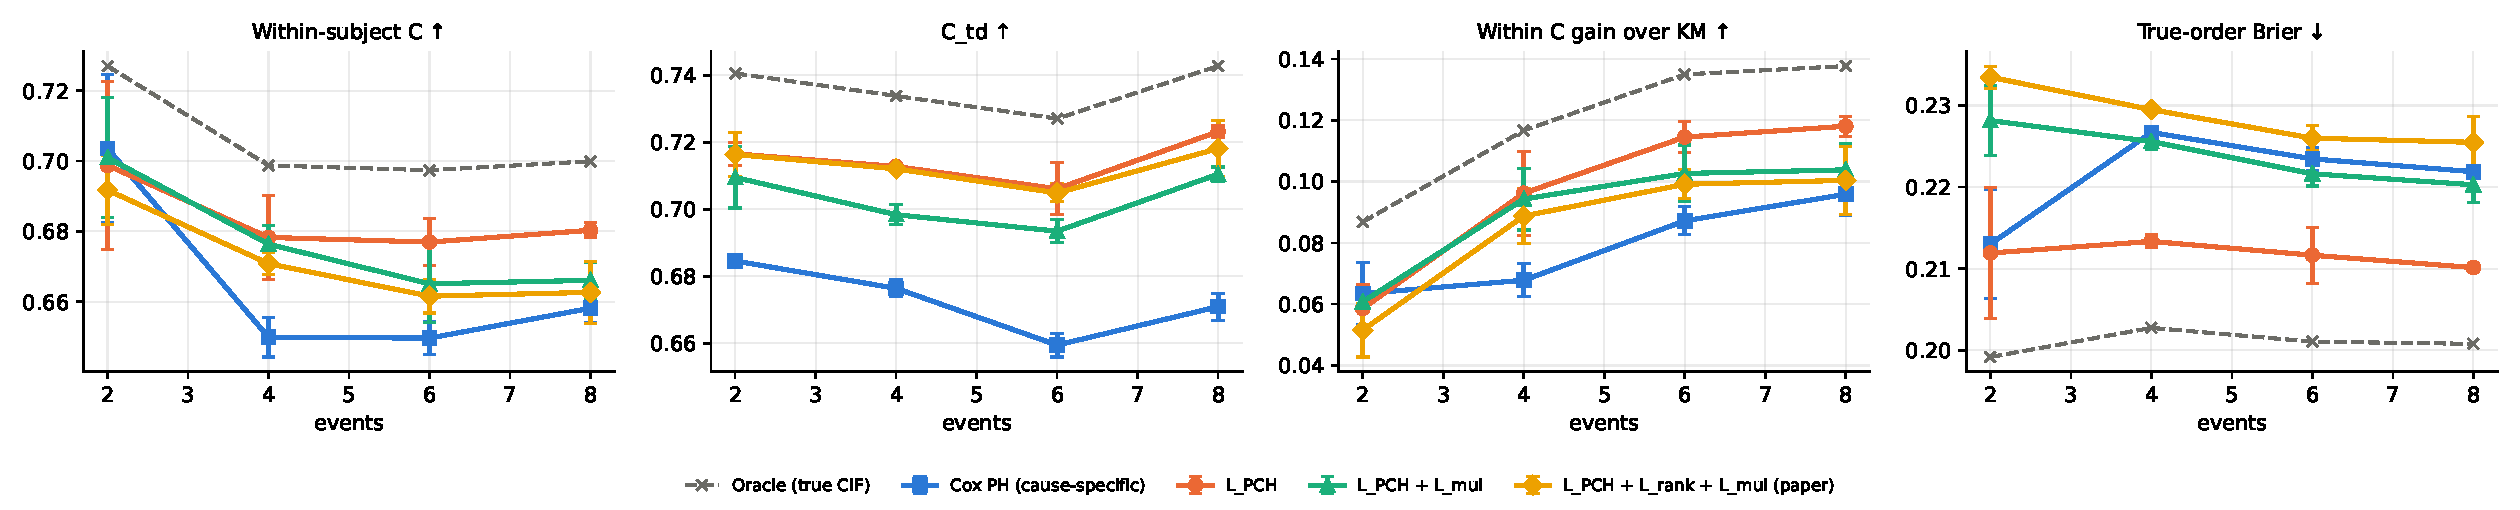
\includegraphics[width=\textwidth]{figures/sweep_events.pdf}
\caption{Number of events $K$ (2 to 8).}\label{fig:events}
\end{figure}
\paragraph{Figure~\ref{fig:events}.} Our model stays $\approx0.02$ below the oracle for every $K$ while Cox stays
0.05--0.07 below: the framework scales with the number of events. \Lmul{} and the paper recipe are below \Lpch{}
on true-order Brier at every $K$ (e.g.\ 0.226 / 0.230 vs.\ 0.213 at $K{=}4$).

\begin{figure}[H]\centering
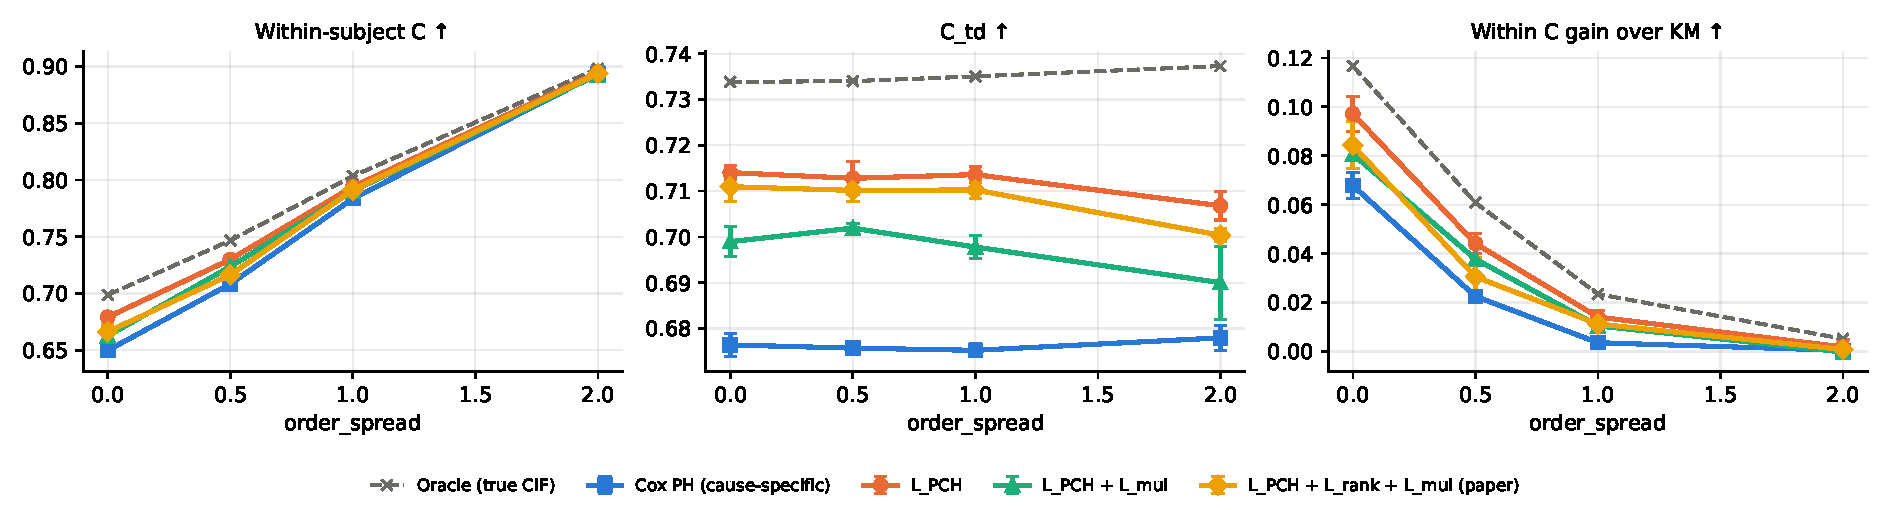
\includegraphics[width=\textwidth]{figures/sweep_order_spread.pdf}
\caption{Spread of the events' typical timing (0 = the patient's covariates decide the order, 2 = nearly the same
order for everybody).}\label{fig:spread}
\end{figure}
\paragraph{Figure~\ref{fig:spread}.} When the order is population-wide (spread 2) every model reaches the oracle's
within-C ($\approx0.89$--$0.90$) and there is nothing patient-specific to learn (gain $\approx0$). When the order is
patient-specific (spread 0) the oracle reaches 0.699, \Lpch{} 0.679 and \Lmul{} 0.663 --- \Lmul{} is lower exactly
where it was meant to help.

\begin{figure}[H]\centering
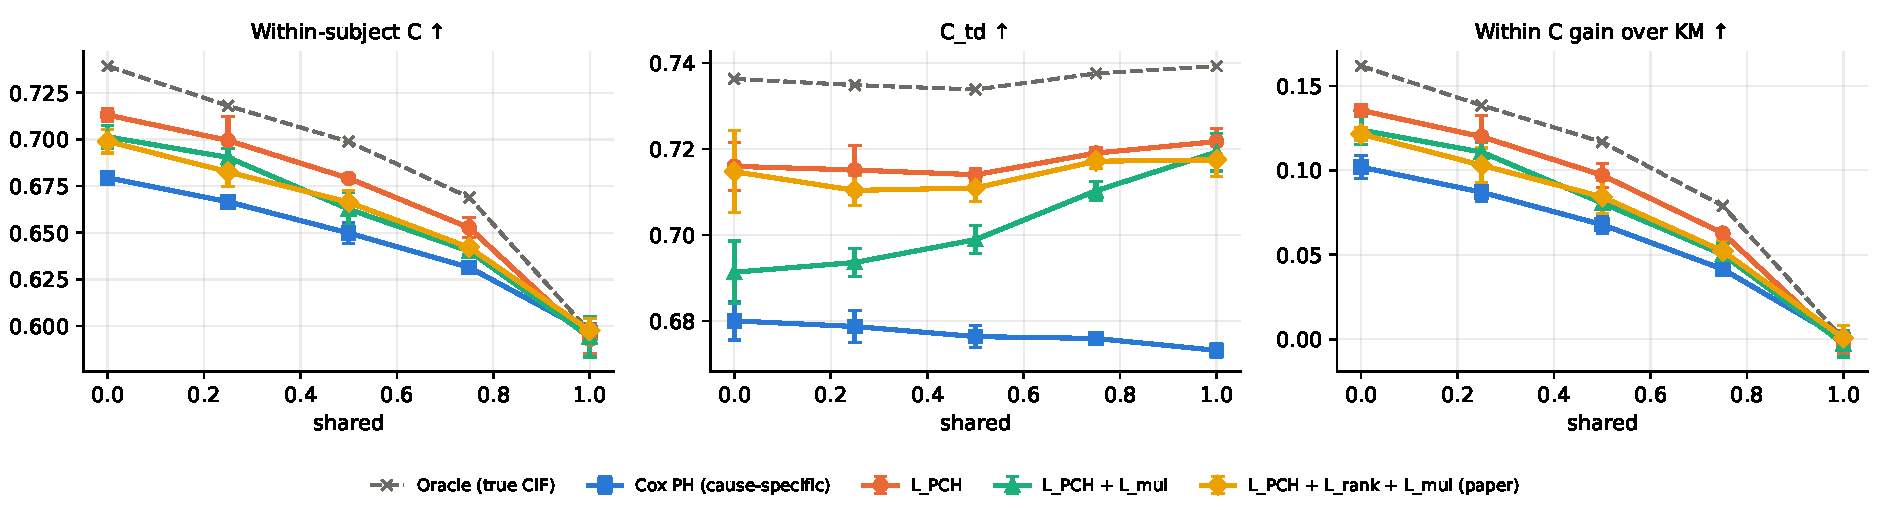
\includegraphics[width=\textwidth]{figures/sweep_shared.pdf}
\caption{Share of the risk common to all events (``shared disease pathway'').}\label{fig:shared}
\end{figure}
\paragraph{Figure~\ref{fig:shared}.} With more shared risk there is less patient-specific ordering to learn; at
shared $=1$ even the oracle gains nothing over population ordering (0.000), confirming the metric behaves as
intended in the non-competing regime. Our model tracks the oracle at every level; \Lmul{} is never above \Lpch{}.

\begin{figure}[H]\centering
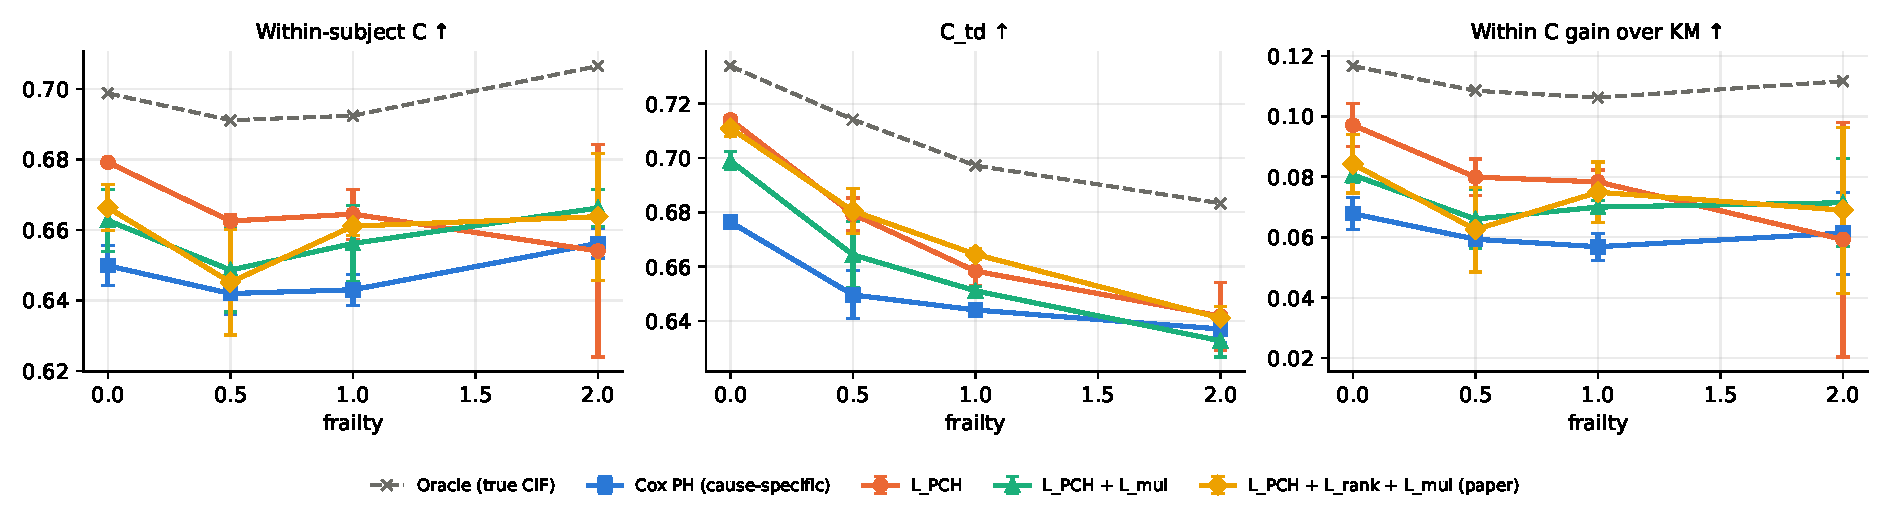
\includegraphics[width=\textwidth]{figures/sweep_frailty.pdf}
\caption{Unobserved shared frailty (dependence covariates cannot explain).}\label{fig:frailty}
\end{figure}
\paragraph{Figure~\ref{fig:frailty}.} Frailty lowers every model and the oracle together (C$_{td}$ of \Lpch{} 0.714
$\to$ 0.642 at variance 2); no loss variant is more robust than \Lpch{}.

\begin{figure}[H]\centering
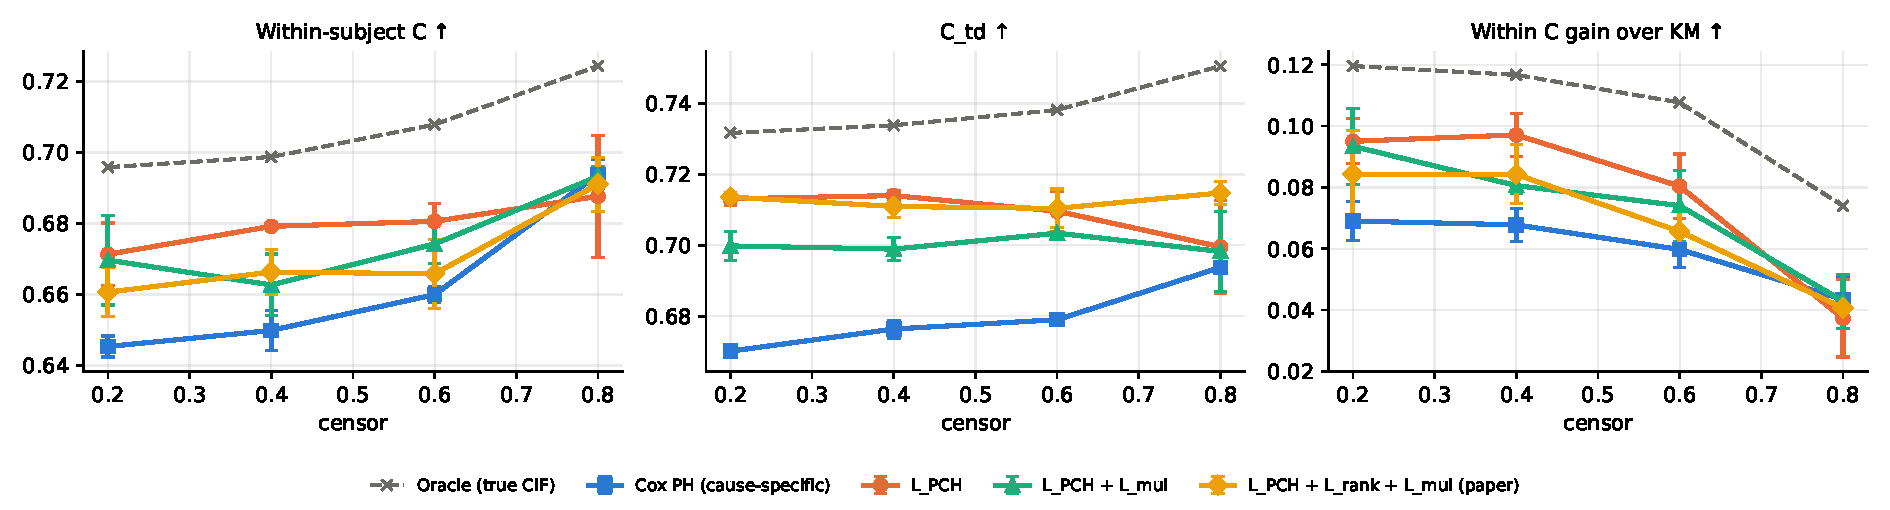
\includegraphics[width=\textwidth]{figures/sweep_censor.pdf}
\caption{Fraction of unobserved event slots (censoring).}\label{fig:censor}
\end{figure}
\paragraph{Figure~\ref{fig:censor}.} Performance is stable from 20\,\% to 80\,\% censoring (\Lpch{} C$_{td}$
0.700--0.714); the ordering of models does not change.

\begin{figure}[H]\centering
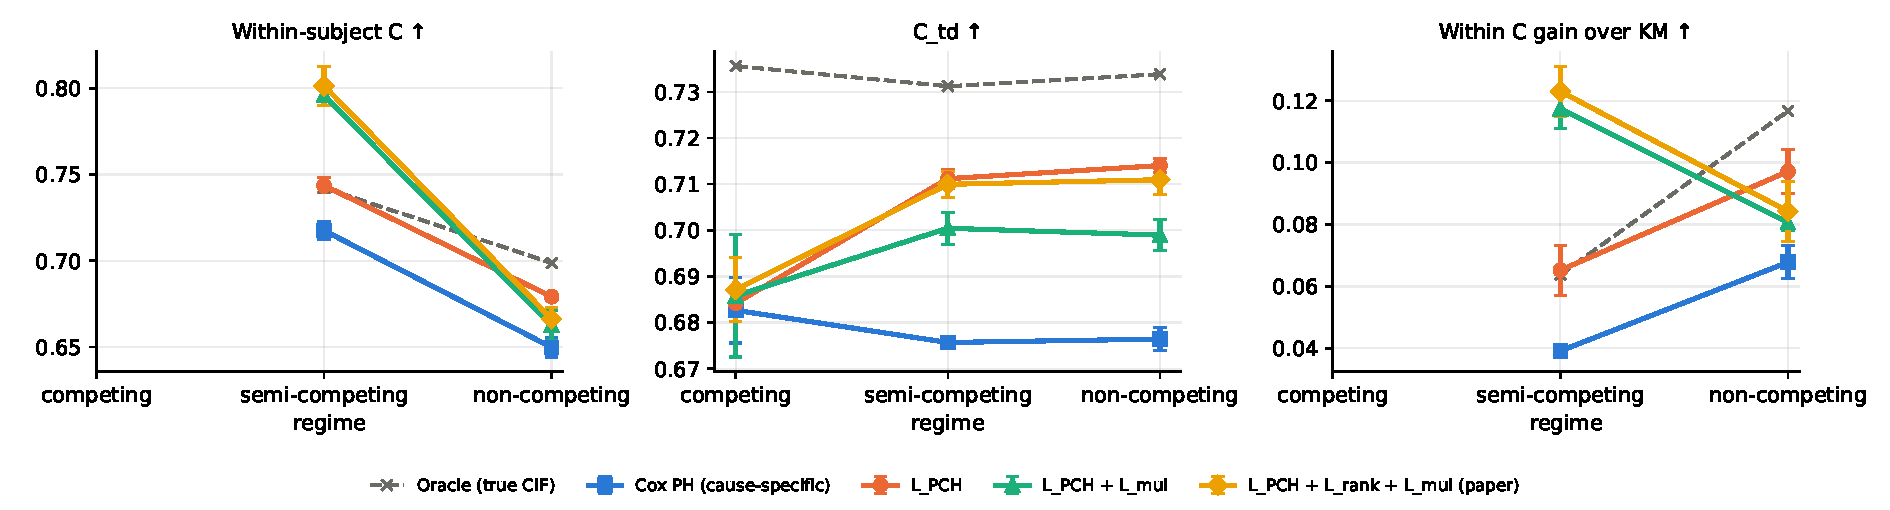
\includegraphics[width=\textwidth]{figures/sweep_regime.pdf}
\caption{Observation regime.}\label{fig:regime}
\end{figure}
\paragraph{Figure~\ref{fig:regime}.} Under competing risks only the first event is observed, so there are no
orderable pairs and within-C is undefined. Under semi-competing risks \Lmul{} and the paper recipe reach within-C
0.796--0.802, far above the oracle's 0.742: the first sign of the gaming confirmed in Table~\ref{tab:true}.
C$_{td}$ is similar across regimes ($\approx0.70$--$0.71$ for our model).

%=====================================================================
\section{Continuous vs.\ discretised numeric input (notebook 10)}
%=====================================================================
\begin{table}[H]\centering\small
\caption{Same model and splits, numeric features standardised (continuous) or cut into 10 quantile bins. C$_{td}$, 5 splits.
SUPPORT ``continuous'' is affected by the preprocessing issue noted on page~1 (the discretised path is not).}
\label{tab:disc}
\begin{tabular}{lcccc}
\toprule
 & \multicolumn{2}{c}{METABRIC} & \multicolumn{2}{c}{SUPPORT} \\
\cmidrule(lr){2-3}\cmidrule(lr){4-5}
Model & continuous & discretised & continuous & discretised \\
\midrule
Ours \Lpch{} & \best{0.675}\,$\pm$\,0.011 & 0.652\,$\pm$\,0.018 & 0.609\,$\pm$\,0.009 & \best{0.621}\,$\pm$\,0.010 \\
DeepHit & \best{0.675}\,$\pm$\,0.010 & 0.654\,$\pm$\,0.019 & 0.603\,$\pm$\,0.009 & \best{0.625}\,$\pm$\,0.005 \\
\bottomrule
\end{tabular}
\end{table}
\paragraph{Reading Table~\ref{tab:disc}.} Continuous input is better on METABRIC ($+0.023$) and discretised input
is better on SUPPORT ($+0.012$ to $+0.022$), for both models. Part or all of the SUPPORT difference is explained
by the preprocessing issue noted on page~1: on the continuous path five SUPPORT measurements were unscaled and one
was lost, while the discretised path was correct. The corrected comparison, including a quantile (rank) transform,
is in notebook 12. The paper should not claim continuous encoding is always better; a rank/quantile
transform before the value embedding is a cheap candidate to get both.

%=====================================================================
\section{Coded visit histories, \S4.2 (notebooks 06 and 09)}
%=====================================================================
\begin{table}[H]\centering\small
\caption{The same patients given to our model as the full time-stamped sequence, a bag-of-codes table (counts, last
lab values, number of visits) or static features only. C$_{td}$, 3 splits. ``temporal'' = share of risk carried by
order, trend and recency.}
\label{tab:ehr}
\resizebox{\textwidth}{!}{\begin{tabular}{llcccccc}
\toprule
Design & cohort & Oracle & Cox [bag] & Ours [bag] & Ours [sequence] & MENSA [seq.] & Ours [static] \\
\midrule
v1 & static (0.0) & 0.735 & 0.725 & 0.710 & 0.708 & 0.712 & 0.502 \\
v1 & base (0.5) & 0.723 & 0.708 & 0.705 & 0.700 & 0.690 & 0.500 \\
v1 & temporal (0.9) & 0.708 & 0.688 & 0.686 & 0.684 & 0.675 & 0.500 \\
\midrule
v2 & level (0.0) & 0.745 & 0.735 & 0.716 & 0.726 & 0.721 & 0.502 \\
v2 & mixed (0.5) & 0.725 & 0.697 & 0.691 & 0.687 & 0.681 & 0.498 \\
v2 & order (0.9) & 0.696 & 0.653 & 0.655 & 0.647 & 0.645 & 0.502 \\
\bottomrule
\end{tabular}}
\end{table}
\paragraph{Reading Table~\ref{tab:ehr}.} In v1 the temporal signal could be recovered from counts and last values
(a linear model on the bag recovers 66--86\,\% of the true risk), so sequence and bag tie. v2 removes this shortcut
(the bag recovers only 12--41\,\% for three of four outcomes), and the oracle's lead over every model grows with
the temporal share (0.010 $\to$ 0.043): the extra information is there. No model extracts it: our sequence model
stays at the bag level (0.647 vs.\ 0.655 in the ``order'' cohort). Likely causes are the very small transformer
(hidden size 16, 2 layers), mean pooling over up to 256 mostly-noise tokens, time entering only as the value of a
\texttt{VISIT} token, and $\approx$3\,000 training patients. Static input (age and sex) is at chance, as designed.
\S4.2 is therefore not supported yet. On these data DeepHit again orders events badly (within-C 0.41--0.47).

%=====================================================================
\section{End-to-end LLM, \S3 (notebooks 05 and 07)}
%=====================================================================
\begin{table}[H]\centering\small
\caption{The \S3 language model vs.\ Cox and our transformer on the same splits. C$_{td}$, 3 splits.}
\label{tab:llm}
\begin{tabular}{lccc}
\toprule
Model & sim\_base & EBMT & METABRIC \\
\midrule
Oracle & 0.734 & -- & -- \\
Cox PH & 0.676 & 0.538 & 0.624 \\
Ours \Lpch{} & \best{0.713} & 0.544 & 0.666 \\
Ours paper recipe & 0.709 & 0.544 & \best{0.676} \\
LLM, DistilGPT2 pretrained & 0.621\,$\pm$\,0.060 & \best{0.550} & 0.589\,$\pm$\,0.038 \\
LLM, GPT-2 from scratch & 0.654\,$\pm$\,0.012 & 0.538 & 0.544\,$\pm$\,0.055 \\
\bottomrule
\end{tabular}
\end{table}
\paragraph{Reading Table~\ref{tab:llm}.} The LLM formulation works end to end and is clearly above chance, but it is
weaker than our transformer by 0.06--0.08 on sim\_base and METABRIC; on EBMT, where every model is near 0.54, it
ties. The pretrained model is unstable across splits (sd up to 0.06). It is best presented as a proof of concept.

%=====================================================================
\section{What we know now}
%=====================================================================
\begin{enumerate}
  \item The transformer with the \Lpch{} likelihood is the best or tied-best of the models we ran on METABRIC,
        SUPPORT, hsa\_synthetic, EBMT and the simulator, with the best calibration among neural models
        (Tables~\ref{tab:single}, \ref{tab:multi}); it is below the published SurvTRACE on METABRIC and SUPPORT. On the
        synthetic EHR cohorts, whose risk is close to linear in the bag-of-codes features, Cox on the bag table is
        equal or better (Table~\ref{tab:ehr}).
  \item Measured against the true event order, it orders events within a patient better than every other learned
        model; the competing-risk DeepHit is worst (Table~\ref{tab:true}). This supports the general multi-event
        formulation.
  \item \Lrank{} and \Lmul{} do not improve any proper score, tuned or not (Tables~\ref{tab:true}, \ref{tab:tune};
        Figures~\ref{fig:events} and~\ref{fig:spread}).
  \item The within-subject C-index rewards a loss trained on it beyond the oracle (Table~\ref{tab:true},
        Figure~\ref{fig:regime}); proper true-order scores are needed to evaluate multi-event models.
  \item The neural model pays off for non-linear signal and clearly from $\approx$5\,000 subjects; it scales to 8 events
        (Figures~\ref{fig:nonlin}--\ref{fig:events}).
  \item MMV trades calibration for lower error on observed event times; useful only when time accuracy matters.
  \item Continuous vs.\ discretised input is dataset-dependent (Table~\ref{tab:disc}).
  \item Coded sequences do not yet beat a bag of codes although the signal is present (Table~\ref{tab:ehr}).
  \item The end-to-end LLM works but is weaker (Table~\ref{tab:llm}).
\end{enumerate}

\section{Open items}
Ordered by how much each could change the paper's claims.
\begin{enumerate}
  \item \textbf{Corrected SUPPORT results.} Re-run of the SUPPORT benchmark and of the
        encoding comparison with the fixed preprocessing (notebook 12); this also re-opens the gap to SurvTRACE on SUPPORT.
  \item \textbf{Coded sequences (\S4.2).} The v2 cohorts show the information is in the history but our model does
        not extract it. Planned: a larger transformer, attention or \texttt{[CLS]} pooling instead of mean pooling,
        an explicit time encoding, and more training patients; then re-run notebook 09. This is the one negative
        result that could still turn into support for the paper.
  \item \textbf{Gap to the published SurvTRACE.} Our model is 0.016 (METABRIC) and 0.032 (SUPPORT) below it.
        The backbone is already tuned per dataset; what remains is SurvTRACE's multi-task head (worth
        0.004--0.005 in their own ablation) and a comparison on identical splits before claiming parity.
  \item \textbf{Numeric encoding.} Continuous input wins on METABRIC and quantile bins win on SUPPORT; a
        rank/quantile transform before the value embedding may give both.
  \item \textbf{Role of \Lrank{}/\Lmul{} in the paper.} The evidence says they are neutral when tuned and harmful
        when sharp. The paper should either present them as optional penalties with this ablation, or drop the claim
        that they improve prediction.
  \item \textbf{Evaluation of multi-event models.} The within-subject C-index is gameable; the true-order scores
        (Section~\ref{sec:true}) should replace it in the paper, which is also a methodological contribution.
  \item \textbf{Real multi-event data with richer covariates.} EBMT has only four categorical covariates. MIMIC needs
        PhysioNet credentialing; the \S4.2 CKD/COPD/diabetes cohorts can be loaded through \texttt{patients.csv} and
        \texttt{events.csv} once available.
  \item \textbf{Manuscript corrections.} The sign of $\eta$ in Eqs.~4--5 (the code is correct), a MENSA row in
        Table~1 of the paper, and the end-to-end LLM presented as a proof of concept.
\end{enumerate}

\appendix
\section{Where the numbers come from}
\begin{center}\small
\begin{tabular}{ll}
\toprule
Table / figure & source (\texttt{results/new\_results/}) \\
\midrule
Table~\ref{tab:single} & \texttt{03\_single\_event\_benchmarks/report} \\
Table~\ref{tab:multi} & \texttt{01\_multievent\_lmul/report}, \texttt{07\_rerun\_failed/report} \\
Tables~\ref{tab:true}, \ref{tab:tune} & \texttt{08\_true\_order\_and\_tuning} (tuned and untuned runs separated by tag) \\
Figures~\ref{fig:spread}--\ref{fig:regime} & \texttt{02\_synthetic\_scenarios/report/sweep\_*} \\
Figures~\ref{fig:nonlin}--\ref{fig:events} & \texttt{11\_extra\_sweeps/report/sweep\_*} \\
Table~\ref{tab:disc} & \texttt{10\_continuous\_vs\_discretised/report} \\
Table~\ref{tab:ehr} & \texttt{06\_sequential\_ehr/report}, \texttt{09\_sequential\_ehr\_v2/report} \\
Table~\ref{tab:llm} & \texttt{05\_llm\_end\_to\_end/report}, \texttt{07\_rerun\_failed/report} \\
\bottomrule
\end{tabular}
\end{center}
\end{document}
